\documentclass[handout]{beamer}
\usepackage{array}
\usepackage{german}
\usepackage{graphicx}
\usepackage[utf8]{inputenc}
\usepackage[T1]{fontenc}
\mode<beamer>{%
\usetheme{Copenhagen}
}
\usepackage[orientation=landscape,size=a3,debug,scale=2.9]{beamerposter}
\title[]{}
\begin{document}
\begin{frame}
\frametitle{MathSem 2019: Wavelets}
\begin{columns}[onlytextwidth]
\begin{column}{0.32\textwidth}
{\bf\large Das Buch zum Seminar}
\bigskip
\vskip 1cm
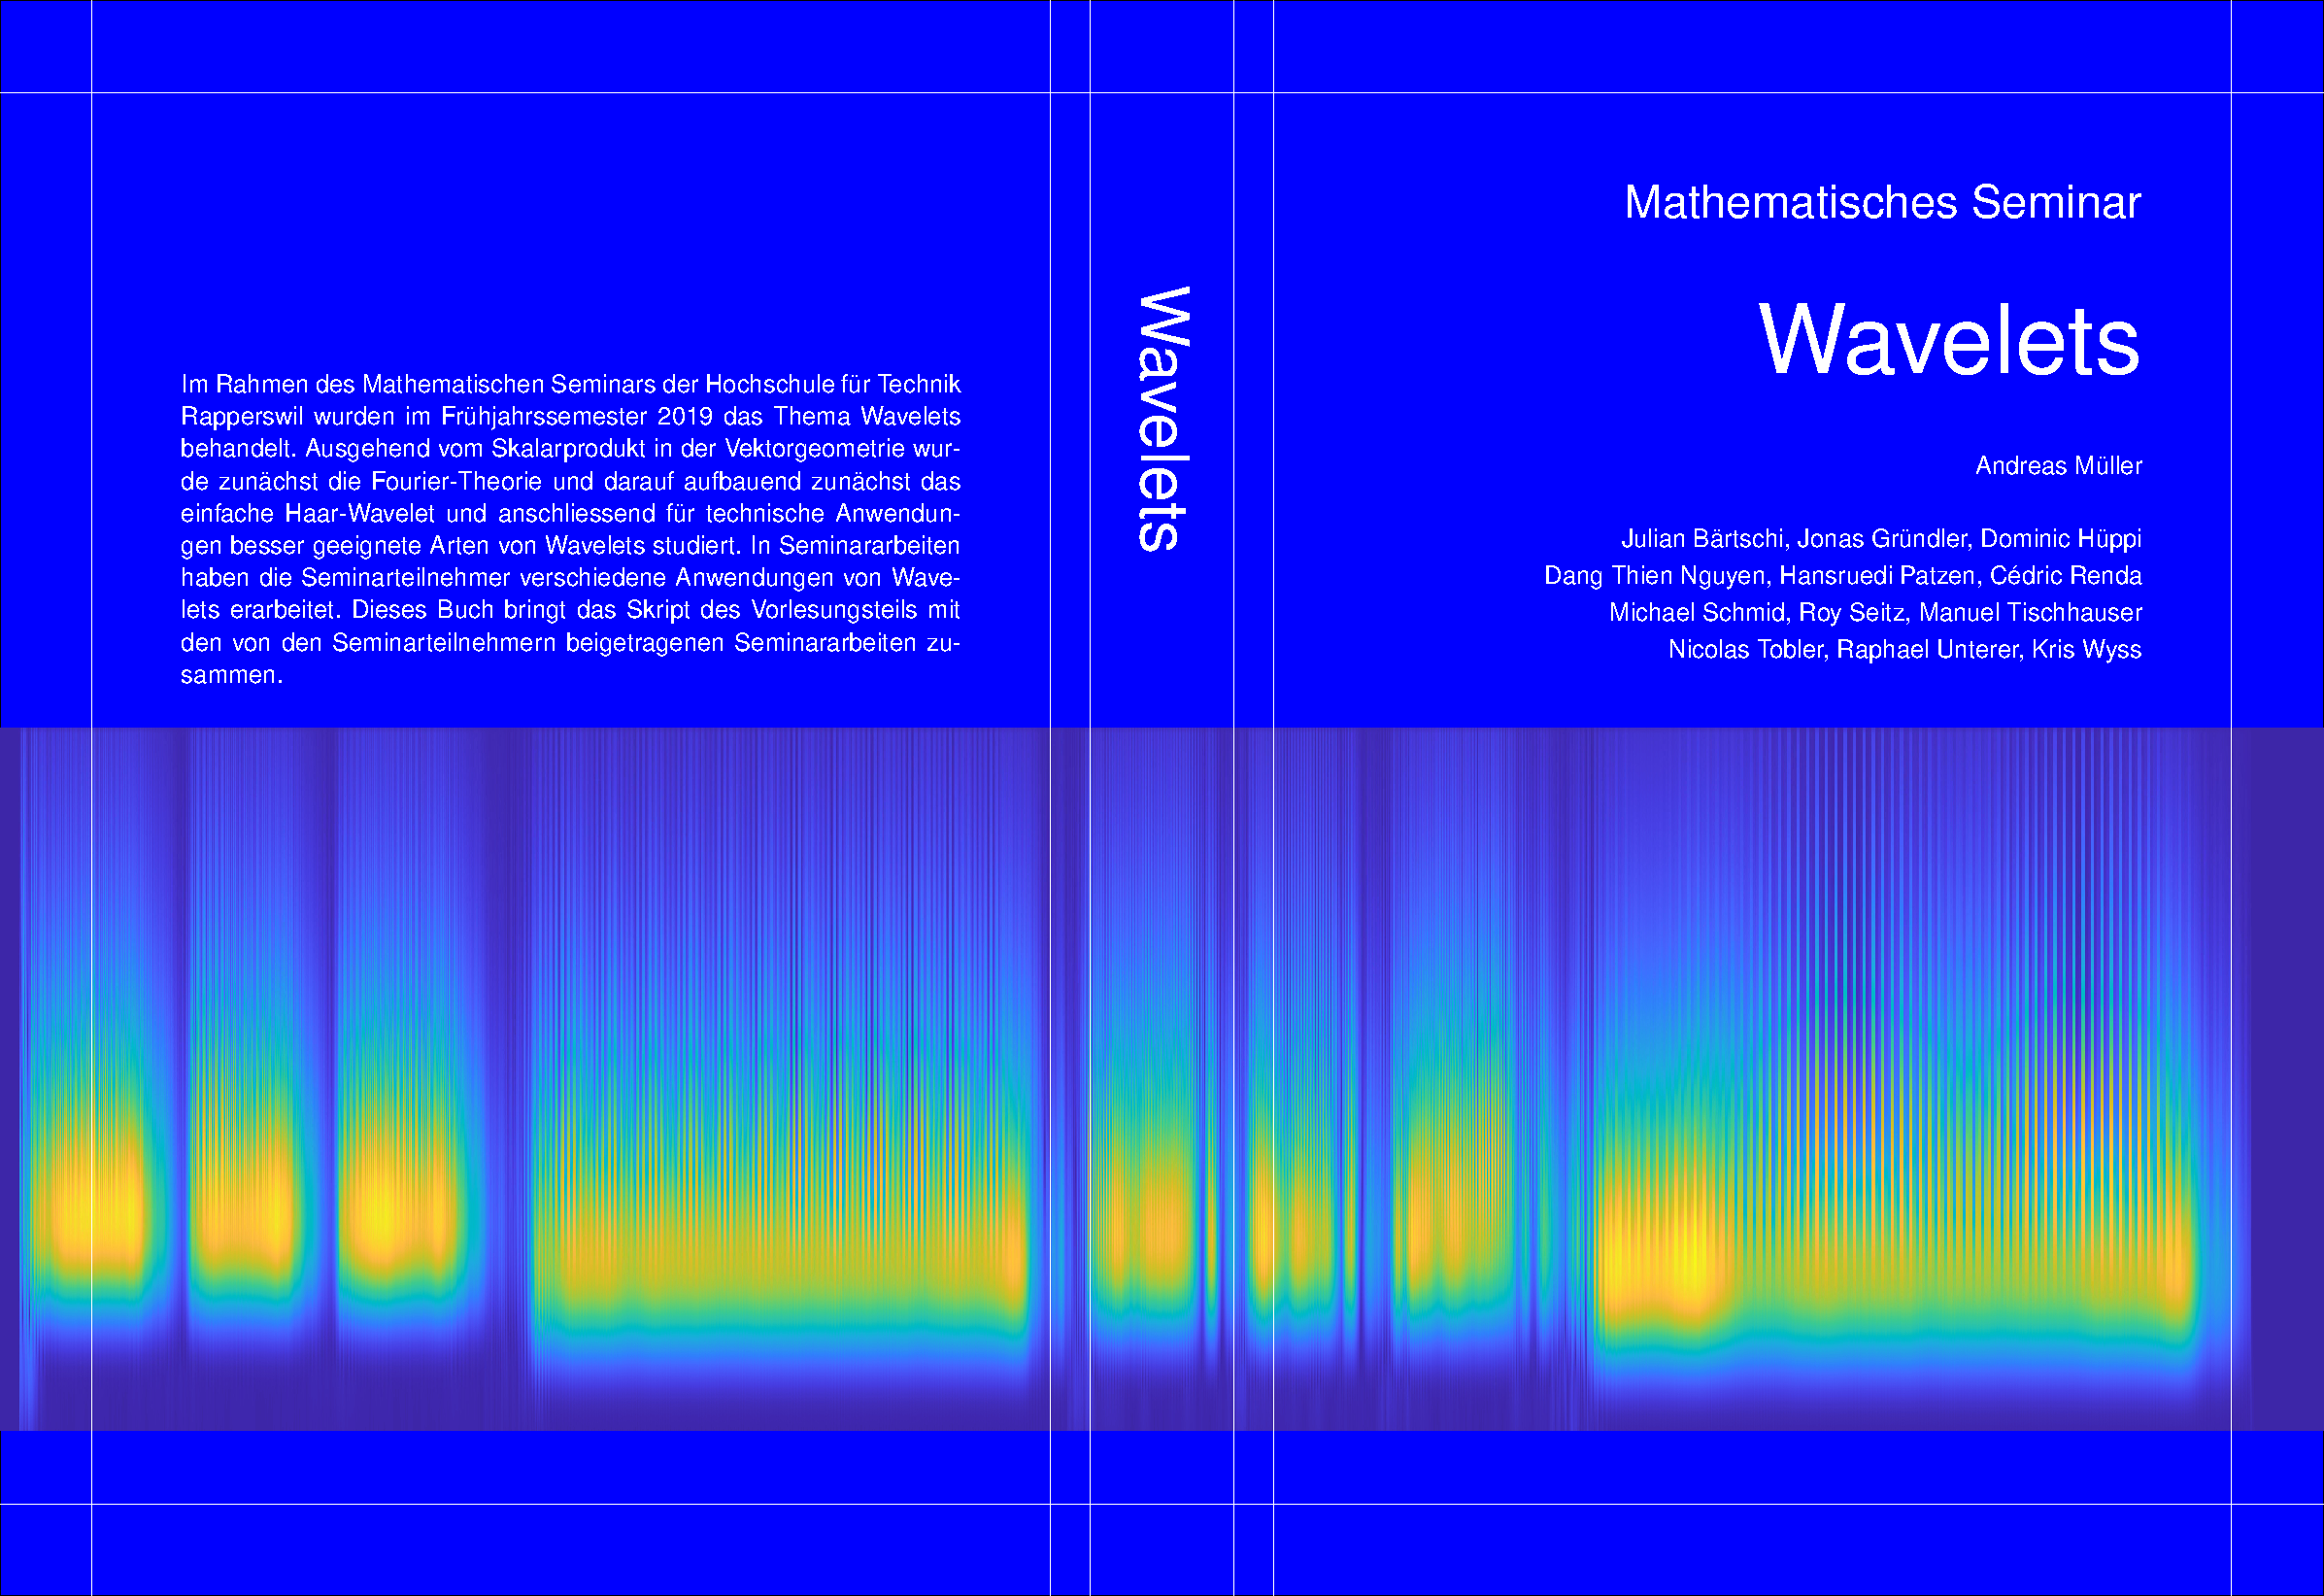
\includegraphics[width=\hsize]{../cover/buchcover.png}
\vskip 0.2cm
%\bigskip
%\bigskip
%\bigskip
Erscheint im Sommer 2019.
Anfragen an
Prof.~Dr.~Andreas Müller,
{\texttt{andreas.mueller@hsr.ch}}
\end{column}
\begin{column}{0.63\textwidth}
\begin{description}
\item[Teil 1:] Grundlagen
\begin{enumerate}
\item Sampling und Geometrie
\item Fouriertheorie und die $L^2$-Hilberträume
\item Das Haar-Wavelet
\item Stetige Wavelet-Transformation
\item Abtast-Theorem und Rekonstruktion
\item Multiskalen-Analyse
\item Schnelle Wavelet-Algorithmen
\item Wavelets mit kompaktem Träger
\item Spline-Wavelets
\end{enumerate}
\item[Teil 2:] Anwendungen und weiterführende Themen
\begin{enumerate}
\setcounter{enumi}{9}
\item Cédric Renda: {\em Autotune}
\item Manuel Tischhauser: {\em Wavelet-Deconvolution}
\item Nicolas Tobler und Jonas Gründler: {\em FPGA-Implementation der
schnellen Wavelet-Transformation}
\item Julian Bärtschi: {\em Audio-Kompression mit Daubechies-Wavelets}
\item Raphael Unterer: {\em Gabor-Wavelets und visuelle Wahrnehmung}
\item Roy Seitz: {\em Komplexe Analysis und Wavelets}
\item Raphael Nestler: {\em 2D-Wavelets und Oberflächen}
\item Kris Wyss: {\em Signalanalyse in GIS}
\item Dominique Hüppi: {\em Analyse von Meteor-Echos}
\item Michael Schmid: {\em Wetter-Wavelet-Transformation}
\end{enumerate}
\end{description}
\end{column}
\end{columns}
\end{frame}
\end{document}
